\documentclass[twoside]{book}

% Packages required by doxygen
\usepackage{fixltx2e}
\usepackage{calc}
\usepackage{doxygen}
\usepackage[export]{adjustbox} % also loads graphicx
\usepackage{graphicx}
\usepackage[utf8]{inputenc}
\usepackage{makeidx}
\usepackage{multicol}
\usepackage{multirow}
\PassOptionsToPackage{warn}{textcomp}
\usepackage{textcomp}
\usepackage[nointegrals]{wasysym}
\usepackage[table]{xcolor}

% Font selection
\usepackage[T1]{fontenc}
\usepackage[scaled=.90]{helvet}
\usepackage{courier}
\usepackage{amssymb}
\usepackage{sectsty}
\renewcommand{\familydefault}{\sfdefault}
\allsectionsfont{%
  \fontseries{bc}\selectfont%
  \color{darkgray}%
}
\renewcommand{\DoxyLabelFont}{%
  \fontseries{bc}\selectfont%
  \color{darkgray}%
}
\newcommand{\+}{\discretionary{\mbox{\scriptsize$\hookleftarrow$}}{}{}}

% Page & text layout
\usepackage{geometry}
\geometry{%
  a4paper,%
  top=2.5cm,%
  bottom=2.5cm,%
  left=2.5cm,%
  right=2.5cm%
}
\tolerance=750
\hfuzz=15pt
\hbadness=750
\setlength{\emergencystretch}{15pt}
\setlength{\parindent}{0cm}
\setlength{\parskip}{3ex plus 2ex minus 2ex}
\makeatletter
\renewcommand{\paragraph}{%
  \@startsection{paragraph}{4}{0ex}{-1.0ex}{1.0ex}{%
    \normalfont\normalsize\bfseries\SS@parafont%
  }%
}
\renewcommand{\subparagraph}{%
  \@startsection{subparagraph}{5}{0ex}{-1.0ex}{1.0ex}{%
    \normalfont\normalsize\bfseries\SS@subparafont%
  }%
}
\makeatother

% Headers & footers
\usepackage{fancyhdr}
\pagestyle{fancyplain}
\fancyhead[LE]{\fancyplain{}{\bfseries\thepage}}
\fancyhead[CE]{\fancyplain{}{}}
\fancyhead[RE]{\fancyplain{}{\bfseries\leftmark}}
\fancyhead[LO]{\fancyplain{}{\bfseries\rightmark}}
\fancyhead[CO]{\fancyplain{}{}}
\fancyhead[RO]{\fancyplain{}{\bfseries\thepage}}
\fancyfoot[LE]{\fancyplain{}{}}
\fancyfoot[CE]{\fancyplain{}{}}
\fancyfoot[RE]{\fancyplain{}{\bfseries\scriptsize Generated by Doxygen }}
\fancyfoot[LO]{\fancyplain{}{\bfseries\scriptsize Generated by Doxygen }}
\fancyfoot[CO]{\fancyplain{}{}}
\fancyfoot[RO]{\fancyplain{}{}}
\renewcommand{\footrulewidth}{0.4pt}
\renewcommand{\chaptermark}[1]{%
  \markboth{#1}{}%
}
\renewcommand{\sectionmark}[1]{%
  \markright{\thesection\ #1}%
}

% Indices & bibliography
\usepackage{natbib}
\usepackage[titles]{tocloft}
\setcounter{tocdepth}{3}
\setcounter{secnumdepth}{5}
\makeindex

% Hyperlinks (required, but should be loaded last)
\usepackage{ifpdf}
\ifpdf
  \usepackage[pdftex,pagebackref=true]{hyperref}
\else
  \usepackage[ps2pdf,pagebackref=true]{hyperref}
\fi
\hypersetup{%
  colorlinks=true,%
  linkcolor=blue,%
  citecolor=blue,%
  unicode%
}

% Custom commands
\newcommand{\clearemptydoublepage}{%
  \newpage{\pagestyle{empty}\cleardoublepage}%
}

\usepackage{caption}
\captionsetup{labelsep=space,justification=centering,font={bf},singlelinecheck=off,skip=4pt,position=top}

%===== C O N T E N T S =====

\begin{document}

% Titlepage & ToC
\hypersetup{pageanchor=false,
             bookmarksnumbered=true,
             pdfencoding=unicode
            }
\pagenumbering{alph}
\begin{titlepage}
\vspace*{7cm}
\begin{center}%
{\Large My Project }\\
\vspace*{1cm}
{\large Generated by Doxygen 1.8.13}\\
\end{center}
\end{titlepage}
\clearemptydoublepage
\pagenumbering{roman}
\tableofcontents
\clearemptydoublepage
\pagenumbering{arabic}
\hypersetup{pageanchor=true}

%--- Begin generated contents ---
\chapter{Namespace Index}
\section{Namespace List}
Here is a list of all documented namespaces with brief descriptions\+:\begin{DoxyCompactList}
\item\contentsline{section}{\hyperlink{namespace_b_plus_tree}{B\+Plus\+Tree} }{\pageref{namespace_b_plus_tree}}{}
\end{DoxyCompactList}

\chapter{Hierarchical Index}
\section{Class Hierarchy}
This inheritance list is sorted roughly, but not completely, alphabetically\+:\begin{DoxyCompactList}
\item \contentsline{section}{Collection}{\pageref{class_collection}}{}
\item \contentsline{section}{Field\+:\+:Data}{\pageref{union_field_1_1_data}}{}
\item \contentsline{section}{Database}{\pageref{class_database}}{}
\item \contentsline{section}{Field}{\pageref{struct_field}}{}
\item \contentsline{section}{Field\+Data}{\pageref{union_field_data}}{}
\item \contentsline{section}{Index}{\pageref{class_index}}{}
\item \contentsline{section}{Key}{\pageref{struct_key}}{}
\item \contentsline{section}{B\+Plus\+Tree\+:\+:Map$<$ K, V $>$}{\pageref{class_b_plus_tree_1_1_map}}{}
\item \contentsline{section}{B\+Plus\+Tree\+:\+:Node$<$ K, V $>$}{\pageref{struct_b_plus_tree_1_1_node}}{}
\item \contentsline{section}{Database\+:\+:Query}{\pageref{class_database_1_1_query}}{}
\item \contentsline{section}{Query\+Option\+Data}{\pageref{union_query_option_data}}{}
\item \contentsline{section}{Database\+:\+:Record}{\pageref{class_database_1_1_record}}{}
\item \contentsline{section}{Collection\+:\+:Record}{\pageref{class_collection_1_1_record}}{}
\item runtime\+\_\+error\begin{DoxyCompactList}
\item \contentsline{section}{B\+Plus\+Tree\+:\+:Map$<$ K, V $>$\+:\+:Key\+Error}{\pageref{class_b_plus_tree_1_1_map_1_1_key_error}}{}
\end{DoxyCompactList}
\end{DoxyCompactList}

\chapter{Class Index}
\section{Class List}
Here are the classes, structs, unions and interfaces with brief descriptions\+:\begin{DoxyCompactList}
\item\contentsline{section}{\hyperlink{class_collection}{Collection} }{\pageref{class_collection}}{}
\item\contentsline{section}{\hyperlink{union_field_1_1_data}{Field\+::\+Data} }{\pageref{union_field_1_1_data}}{}
\item\contentsline{section}{\hyperlink{class_database}{Database} }{\pageref{class_database}}{}
\item\contentsline{section}{\hyperlink{struct_field}{Field} }{\pageref{struct_field}}{}
\item\contentsline{section}{\hyperlink{union_field_data}{Field\+Data} }{\pageref{union_field_data}}{}
\item\contentsline{section}{\hyperlink{class_index}{Index} }{\pageref{class_index}}{}
\item\contentsline{section}{\hyperlink{struct_key}{Key} }{\pageref{struct_key}}{}
\item\contentsline{section}{\hyperlink{class_b_plus_tree_1_1_map_1_1_key_error}{B\+Plus\+Tree\+::\+Map$<$ K, V $>$\+::\+Key\+Error} }{\pageref{class_b_plus_tree_1_1_map_1_1_key_error}}{}
\item\contentsline{section}{\hyperlink{class_b_plus_tree_1_1_map}{B\+Plus\+Tree\+::\+Map$<$ K, V $>$} }{\pageref{class_b_plus_tree_1_1_map}}{}
\item\contentsline{section}{\hyperlink{struct_b_plus_tree_1_1_node}{B\+Plus\+Tree\+::\+Node$<$ K, V $>$} }{\pageref{struct_b_plus_tree_1_1_node}}{}
\item\contentsline{section}{\hyperlink{class_database_1_1_query}{Database\+::\+Query} }{\pageref{class_database_1_1_query}}{}
\item\contentsline{section}{\hyperlink{union_query_option_data}{Query\+Option\+Data} }{\pageref{union_query_option_data}}{}
\item\contentsline{section}{\hyperlink{class_database_1_1_record}{Database\+::\+Record} }{\pageref{class_database_1_1_record}}{}
\item\contentsline{section}{\hyperlink{class_collection_1_1_record}{Collection\+::\+Record} }{\pageref{class_collection_1_1_record}}{}
\end{DoxyCompactList}

\chapter{Namespace Documentation}
\hypertarget{namespace_b_plus_tree}{}\section{B\+Plus\+Tree Namespace Reference}
\label{namespace_b_plus_tree}\index{B\+Plus\+Tree@{B\+Plus\+Tree}}
\subsection*{Classes}
\begin{DoxyCompactItemize}
\item 
class \hyperlink{class_b_plus_tree_1_1_map}{Map}
\item 
struct \hyperlink{struct_b_plus_tree_1_1_node}{Node}
\end{DoxyCompactItemize}


\subsection{Detailed Description}
A Namespace containing the \hyperlink{class_b_plus_tree_1_1_map}{Map} class 
\chapter{Class Documentation}
\hypertarget{class_collection}{}\section{Collection Class Reference}
\label{class_collection}\index{Collection@{Collection}}
\subsection*{Classes}
\begin{DoxyCompactItemize}
\item 
class \hyperlink{class_collection_1_1_record}{Record}
\end{DoxyCompactItemize}
\subsection*{Public Member Functions}
\begin{DoxyCompactItemize}
\item 
\hyperlink{class_collection_af4c8b62d3038e1ba081aef0c4ebd912d}{Collection} (const std\+::string \&file\+\_\+name)
\item 
\mbox{\Hypertarget{class_collection_a368acd4908fd336e262c8724e2aa6dcf}\label{class_collection_a368acd4908fd336e262c8724e2aa6dcf}} 
{\bfseries Collection} (const \hyperlink{class_collection}{Collection} \&collection)
\item 
void \hyperlink{class_collection_a88502cfa08bc6f1c9eff4974b95d53f3}{sort} (std\+::string output\+\_\+file, std\+::vector$<$ std\+::string $>$ \hyperlink{class_collection_aebff0d78673dac8453ebf51ba32d10eb}{keys})
\item 
\mbox{\Hypertarget{class_collection_acd74867896574ea2ac631ec80f364e96}\label{class_collection_acd74867896574ea2ac631ec80f364e96}} 
void {\bfseries sort} (std\+::string output\+\_\+file, std\+::vector$<$ \hyperlink{struct_key}{Key} $>$ \hyperlink{class_collection_aebff0d78673dac8453ebf51ba32d10eb}{keys})
\item 
std\+::vector$<$ std\+::string $>$ \hyperlink{class_collection_aebff0d78673dac8453ebf51ba32d10eb}{keys} () const
\item 
\mbox{\Hypertarget{class_collection_aa7ca7fea36c577e2067fa70f7d4b2c61}\label{class_collection_aa7ca7fea36c577e2067fa70f7d4b2c61}} 
\hyperlink{class_collection_1_1_record}{Record} {\bfseries get} (size\+\_\+t row)
\item 
\mbox{\Hypertarget{class_collection_a5daca64e8f97ffa565ad18202f724fd6}\label{class_collection_a5daca64e8f97ffa565ad18202f724fd6}} 
\hyperlink{class_collection_1_1_record}{Record} {\bfseries operator\mbox{[}$\,$\mbox{]}} (size\+\_\+t row)
\item 
size\+\_\+t \hyperlink{class_collection_ae6922104df8b79051656b77f5019750f}{size} () const
\end{DoxyCompactItemize}
\subsection*{Public Attributes}
\begin{DoxyCompactItemize}
\item 
\mbox{\Hypertarget{class_collection_a46d269163d5deac053b484cff176bef2}\label{class_collection_a46d269163d5deac053b484cff176bef2}} 
const std\+::string {\bfseries file\+\_\+name}
\end{DoxyCompactItemize}
\subsection*{Static Public Attributes}
\begin{DoxyCompactItemize}
\item 
\mbox{\Hypertarget{class_collection_a3b3dc7b32ffc02b446bd7127015b637b}\label{class_collection_a3b3dc7b32ffc02b446bd7127015b637b}} 
static const size\+\_\+t {\bfseries H\+E\+A\+P\+\_\+\+S\+I\+ZE} = 3
\end{DoxyCompactItemize}
\subsection*{Friends}
\begin{DoxyCompactItemize}
\item 
\mbox{\Hypertarget{class_collection_a697483987cfb91e205b5be2a8f6752c7}\label{class_collection_a697483987cfb91e205b5be2a8f6752c7}} 
class {\bfseries Record}
\end{DoxyCompactItemize}


\subsection{Constructor \& Destructor Documentation}
\mbox{\Hypertarget{class_collection_af4c8b62d3038e1ba081aef0c4ebd912d}\label{class_collection_af4c8b62d3038e1ba081aef0c4ebd912d}} 
\index{Collection@{Collection}!Collection@{Collection}}
\index{Collection@{Collection}!Collection@{Collection}}
\subsubsection{\texorpdfstring{Collection()}{Collection()}}
{\footnotesize\ttfamily Collection\+::\+Collection (\begin{DoxyParamCaption}\item[{const std\+::string \&}]{file\+\_\+name }\end{DoxyParamCaption})}

Constructs \hyperlink{class_collection_af4c8b62d3038e1ba081aef0c4ebd912d}{Collection\+::\+Collection}, initializes file, keys, and index


\begin{DoxyParams}{Parameters}
{\em file\+\_\+name} & \\
\hline
\end{DoxyParams}


\subsection{Member Function Documentation}
\mbox{\Hypertarget{class_collection_aebff0d78673dac8453ebf51ba32d10eb}\label{class_collection_aebff0d78673dac8453ebf51ba32d10eb}} 
\index{Collection@{Collection}!keys@{keys}}
\index{keys@{keys}!Collection@{Collection}}
\subsubsection{\texorpdfstring{keys()}{keys()}}
{\footnotesize\ttfamily std\+::vector$<$std\+::string$>$ Collection\+::keys (\begin{DoxyParamCaption}{ }\end{DoxyParamCaption}) const}

Return a vector of keys available in the associated C\+SV file. The order of the keys also corresponds to the order of keys in a record.

\begin{DoxyReturn}{Returns}
std\+::vector$<$std\+::string$>$ keys 
\end{DoxyReturn}
\mbox{\Hypertarget{class_collection_ae6922104df8b79051656b77f5019750f}\label{class_collection_ae6922104df8b79051656b77f5019750f}} 
\index{Collection@{Collection}!size@{size}}
\index{size@{size}!Collection@{Collection}}
\subsubsection{\texorpdfstring{size()}{size()}}
{\footnotesize\ttfamily size\+\_\+t Collection\+::size (\begin{DoxyParamCaption}{ }\end{DoxyParamCaption}) const}

Return the number of records in a collection

\begin{DoxyReturn}{Returns}
count of records 
\end{DoxyReturn}
\mbox{\Hypertarget{class_collection_a88502cfa08bc6f1c9eff4974b95d53f3}\label{class_collection_a88502cfa08bc6f1c9eff4974b95d53f3}} 
\index{Collection@{Collection}!sort@{sort}}
\index{sort@{sort}!Collection@{Collection}}
\subsubsection{\texorpdfstring{sort()}{sort()}}
{\footnotesize\ttfamily void Collection\+::sort (\begin{DoxyParamCaption}\item[{std\+::string}]{output\+\_\+file,  }\item[{std\+::vector$<$ std\+::string $>$}]{keys }\end{DoxyParamCaption})}

Creates a new sorted C\+SV file at the location {\ttfamily output\+\_\+file} sorted in the order of entries in {\ttfamily keys}.


\begin{DoxyParams}{Parameters}
{\em file\+\_\+name} & \\
\hline
{\em keys} & \\
\hline
\end{DoxyParams}


The documentation for this class was generated from the following file\+:\begin{DoxyCompactItemize}
\item 
include/collection.\+h\end{DoxyCompactItemize}

\hypertarget{union_field_1_1_data}{}\section{Field\+:\+:Data Union Reference}
\label{union_field_1_1_data}\index{Field\+::\+Data@{Field\+::\+Data}}
\subsection*{Public Attributes}
\begin{DoxyCompactItemize}
\item 
\mbox{\Hypertarget{union_field_1_1_data_a3cbf50c722b2632c2c86ce35de9464e1}\label{union_field_1_1_data_a3cbf50c722b2632c2c86ce35de9464e1}} 
int {\bfseries integer}
\item 
\mbox{\Hypertarget{union_field_1_1_data_af5926a75c50c773645711698831c4767}\label{union_field_1_1_data_af5926a75c50c773645711698831c4767}} 
std\+::string $\ast$ {\bfseries string}
\item 
\mbox{\Hypertarget{union_field_1_1_data_a2534986334ffe9070e6ad2b5d74b449e}\label{union_field_1_1_data_a2534986334ffe9070e6ad2b5d74b449e}} 
char $\ast$ {\bfseries str}
\item 
\mbox{\Hypertarget{union_field_1_1_data_afdd5f3468c0f038045c30623ba3f34ea}\label{union_field_1_1_data_afdd5f3468c0f038045c30623ba3f34ea}} 
int {\bfseries num}
\end{DoxyCompactItemize}


The documentation for this union was generated from the following files\+:\begin{DoxyCompactItemize}
\item 
include/collection.\+h\item 
include/record.\+h\end{DoxyCompactItemize}

\hypertarget{class_database}{}\section{Database Class Reference}
\label{class_database}\index{Database@{Database}}
\subsection*{Classes}
\begin{DoxyCompactItemize}
\item 
class \hyperlink{class_database_1_1_query}{Query}
\item 
class \hyperlink{class_database_1_1_record}{Record}
\end{DoxyCompactItemize}
\subsection*{Public Member Functions}
\begin{DoxyCompactItemize}
\item 
\hyperlink{class_database_a0bb07a61d59006f6987bf95e7348a5fa}{Database} (std\+::string filename, D\+B\+Format fmt)
\item 
const \hyperlink{class_database_1_1_record}{Record} \& \hyperlink{class_database_a0ef7dce3f4521e498c574447ed4bfb34}{get} (int n)
\item 
\mbox{\Hypertarget{class_database_af2f845cad2fe104cf26e054858765765}\label{class_database_af2f845cad2fe104cf26e054858765765}} 
\hyperlink{class_database_1_1_query}{Query} {\bfseries query} ()
\end{DoxyCompactItemize}
\subsection*{Public Attributes}
\begin{DoxyCompactItemize}
\item 
\mbox{\Hypertarget{class_database_ac3400745011e67014a4323f7ed84e8be}\label{class_database_ac3400745011e67014a4323f7ed84e8be}} 
const std\+::string {\bfseries filename}
\item 
\mbox{\Hypertarget{class_database_a776c1a8a04c4a79a40860f62d44f9383}\label{class_database_a776c1a8a04c4a79a40860f62d44f9383}} 
const D\+B\+Format {\bfseries format}
\end{DoxyCompactItemize}


\subsection{Constructor \& Destructor Documentation}
\mbox{\Hypertarget{class_database_a0bb07a61d59006f6987bf95e7348a5fa}\label{class_database_a0bb07a61d59006f6987bf95e7348a5fa}} 
\index{Database@{Database}!Database@{Database}}
\index{Database@{Database}!Database@{Database}}
\subsubsection{\texorpdfstring{Database()}{Database()}}
{\footnotesize\ttfamily Database\+::\+Database (\begin{DoxyParamCaption}\item[{std\+::string}]{filename,  }\item[{D\+B\+Format}]{fmt }\end{DoxyParamCaption})}

\hyperlink{class_database_a0bb07a61d59006f6987bf95e7348a5fa}{Database\+::\+Database}


\begin{DoxyParams}{Parameters}
{\em filename} & String of the filename \\
\hline
{\em fmt} & \hyperlink{class_database}{Database} format \\
\hline
\end{DoxyParams}


\subsection{Member Function Documentation}
\mbox{\Hypertarget{class_database_a0ef7dce3f4521e498c574447ed4bfb34}\label{class_database_a0ef7dce3f4521e498c574447ed4bfb34}} 
\index{Database@{Database}!get@{get}}
\index{get@{get}!Database@{Database}}
\subsubsection{\texorpdfstring{get()}{get()}}
{\footnotesize\ttfamily const \hyperlink{class_database_1_1_record}{Record}\& Database\+::get (\begin{DoxyParamCaption}\item[{int}]{n }\end{DoxyParamCaption})}

\hyperlink{class_database_a0ef7dce3f4521e498c574447ed4bfb34}{Database\+::get}


\begin{DoxyParams}{Parameters}
{\em n} & Integer n \\
\hline
\end{DoxyParams}
\begin{DoxyReturn}{Returns}

\end{DoxyReturn}


The documentation for this class was generated from the following file\+:\begin{DoxyCompactItemize}
\item 
include/database.\+h\end{DoxyCompactItemize}

\hypertarget{struct_field}{}\section{Field Class Reference}
\label{struct_field}\index{Field@{Field}}


Collaboration diagram for Field\+:
\nopagebreak
\begin{figure}[H]
\begin{center}
\leavevmode
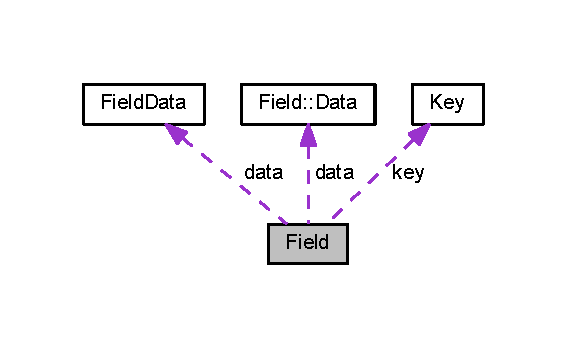
\includegraphics[width=272pt]{struct_field__coll__graph}
\end{center}
\end{figure}
\subsection*{Classes}
\begin{DoxyCompactItemize}
\item 
union \hyperlink{union_field_1_1_data}{Data}
\end{DoxyCompactItemize}
\subsection*{Public Types}
\begin{DoxyCompactItemize}
\item 
\mbox{\Hypertarget{struct_field_ab791686c1600914e014bacad1e6459f1}\label{struct_field_ab791686c1600914e014bacad1e6459f1}} 
enum {\bfseries Type} \{ {\bfseries S\+T\+R\+I\+NG}, 
{\bfseries I\+N\+T\+E\+G\+ER}
 \}
\end{DoxyCompactItemize}
\subsection*{Public Member Functions}
\begin{DoxyCompactItemize}
\item 
\hyperlink{struct_field_a6167eb1c3420a4359f0b5bb541f9be94}{Field} (\hyperlink{union_field_1_1_data}{Data} data, \hyperlink{struct_key}{Key} key)
\item 
\mbox{\Hypertarget{struct_field_a1222497e50e48b3d2350c3a46dd19db4}\label{struct_field_a1222497e50e48b3d2350c3a46dd19db4}} 
{\bfseries Field} (const \hyperlink{struct_field}{Field} \&other)
\item 
std\+::string \hyperlink{struct_field_a75a5e874f066c7877a54e760fdfd4aac}{str} () const
\item 
bool \hyperlink{struct_field_a646b48849ac9d8221aa5f3e57cd8b72f}{operator$<$} (const \hyperlink{struct_field}{Field} \&other) const
\item 
bool \hyperlink{struct_field_a768b337c79d52b58e52340cf546414c0}{operator$>$} (const \hyperlink{struct_field}{Field} \&other) const
\item 
bool \hyperlink{struct_field_a3654ee1d9ec7f5c65eb48c4e37e2e309}{operator$<$=} (const \hyperlink{struct_field}{Field} \&other) const
\item 
bool \hyperlink{struct_field_a6d179b2016926bfd9a9e7785a70038d3}{operator$>$=} (const \hyperlink{struct_field}{Field} \&other) const
\item 
bool \hyperlink{struct_field_a1e63e67061b37ff2539b8f6bc7d5adeb}{operator==} (const \hyperlink{struct_field}{Field} \&other) const
\item 
\mbox{\Hypertarget{struct_field_a24edcb7adb06501ba8d77adcc695d1f3}\label{struct_field_a24edcb7adb06501ba8d77adcc695d1f3}} 
{\bfseries Field} (Field\+Type field, \hyperlink{union_field_data}{Field\+Data} data)
\end{DoxyCompactItemize}
\subsection*{Public Attributes}
\begin{DoxyCompactItemize}
\item 
\mbox{\Hypertarget{struct_field_a2e251a573370e077e756a984fa64256e}\label{struct_field_a2e251a573370e077e756a984fa64256e}} 
const union \hyperlink{union_field_1_1_data}{Field\+::\+Data} {\bfseries data}
\item 
\mbox{\Hypertarget{struct_field_a5f9fc1f0a1b484056c6ad31f424d0486}\label{struct_field_a5f9fc1f0a1b484056c6ad31f424d0486}} 
\hyperlink{struct_key}{Key} {\bfseries key}
\item 
\mbox{\Hypertarget{struct_field_ad59cb237a80abf85696249b63f963f8f}\label{struct_field_ad59cb237a80abf85696249b63f963f8f}} 
const Field\+Type {\bfseries field}
\item 
\mbox{\Hypertarget{struct_field_ac5f5015600d388c8a9b07c17db7de3f0}\label{struct_field_ac5f5015600d388c8a9b07c17db7de3f0}} 
const \hyperlink{union_field_data}{Field\+Data} {\bfseries data}
\item 
\mbox{\Hypertarget{struct_field_a301821a927eb0d25fae0b7f6646199a4}\label{struct_field_a301821a927eb0d25fae0b7f6646199a4}} 
const Type {\bfseries field\+\_\+type}
\item 
\mbox{\Hypertarget{struct_field_a904cabbf52aef88a0e8541db856ee4a7}\label{struct_field_a904cabbf52aef88a0e8541db856ee4a7}} 
union \hyperlink{union_field_1_1_data}{Field\+::\+Data} {\bfseries data}
\end{DoxyCompactItemize}


\subsection{Constructor \& Destructor Documentation}
\mbox{\Hypertarget{struct_field_a6167eb1c3420a4359f0b5bb541f9be94}\label{struct_field_a6167eb1c3420a4359f0b5bb541f9be94}} 
\index{Field@{Field}!Field@{Field}}
\index{Field@{Field}!Field@{Field}}
\subsubsection{\texorpdfstring{Field()}{Field()}}
{\footnotesize\ttfamily Field\+::\+Field (\begin{DoxyParamCaption}\item[{\hyperlink{union_field_1_1_data}{Data}}]{data,  }\item[{\hyperlink{struct_key}{Key}}]{key }\end{DoxyParamCaption})\hspace{0.3cm}{\ttfamily [inline]}}

Construct \hyperlink{struct_field}{Field}


\begin{DoxyParams}{Parameters}
{\em data} & \\
\hline
{\em key} & \\
\hline
\end{DoxyParams}


\subsection{Member Function Documentation}
\mbox{\Hypertarget{struct_field_a646b48849ac9d8221aa5f3e57cd8b72f}\label{struct_field_a646b48849ac9d8221aa5f3e57cd8b72f}} 
\index{Field@{Field}!operator$<$@{operator$<$}}
\index{operator$<$@{operator$<$}!Field@{Field}}
\subsubsection{\texorpdfstring{operator$<$()}{operator<()}}
{\footnotesize\ttfamily bool Field\+::operator$<$ (\begin{DoxyParamCaption}\item[{const \hyperlink{struct_field}{Field} \&}]{other }\end{DoxyParamCaption}) const}

$<$ operator applied to \hyperlink{struct_field}{Field}


\begin{DoxyParams}{Parameters}
{\em other} & \\
\hline
\end{DoxyParams}
\begin{DoxyReturn}{Returns}
this-\/$>$data.\+integer $<$ other.\+data.\+integer, or $\ast$(this-\/$>$data.\+string) $<$ $\ast$(other.\+data.\+string) 
\end{DoxyReturn}
\mbox{\Hypertarget{struct_field_a3654ee1d9ec7f5c65eb48c4e37e2e309}\label{struct_field_a3654ee1d9ec7f5c65eb48c4e37e2e309}} 
\index{Field@{Field}!operator$<$=@{operator$<$=}}
\index{operator$<$=@{operator$<$=}!Field@{Field}}
\subsubsection{\texorpdfstring{operator$<$=()}{operator<=()}}
{\footnotesize\ttfamily bool Field\+::operator$<$= (\begin{DoxyParamCaption}\item[{const \hyperlink{struct_field}{Field} \&}]{other }\end{DoxyParamCaption}) const}

$<$= operator applied to \hyperlink{struct_field}{Field}


\begin{DoxyParams}{Parameters}
{\em other} & \\
\hline
\end{DoxyParams}
\begin{DoxyReturn}{Returns}
!($\ast$this $>$ other) 
\end{DoxyReturn}
\mbox{\Hypertarget{struct_field_a1e63e67061b37ff2539b8f6bc7d5adeb}\label{struct_field_a1e63e67061b37ff2539b8f6bc7d5adeb}} 
\index{Field@{Field}!operator==@{operator==}}
\index{operator==@{operator==}!Field@{Field}}
\subsubsection{\texorpdfstring{operator==()}{operator==()}}
{\footnotesize\ttfamily bool Field\+::operator== (\begin{DoxyParamCaption}\item[{const \hyperlink{struct_field}{Field} \&}]{other }\end{DoxyParamCaption}) const}

== opeartor applied to \hyperlink{struct_field}{Field}


\begin{DoxyParams}{Parameters}
{\em other} & \\
\hline
\end{DoxyParams}
\begin{DoxyReturn}{Returns}
this-\/$>$data.\+integer == other.\+data.\+integer, or $\ast$(this-\/$>$data.\+string) == $\ast$(other.\+data.\+string) 
\end{DoxyReturn}
\mbox{\Hypertarget{struct_field_a768b337c79d52b58e52340cf546414c0}\label{struct_field_a768b337c79d52b58e52340cf546414c0}} 
\index{Field@{Field}!operator$>$@{operator$>$}}
\index{operator$>$@{operator$>$}!Field@{Field}}
\subsubsection{\texorpdfstring{operator$>$()}{operator>()}}
{\footnotesize\ttfamily bool Field\+::operator$>$ (\begin{DoxyParamCaption}\item[{const \hyperlink{struct_field}{Field} \&}]{other }\end{DoxyParamCaption}) const}

\begin{quote}
operator applied to \hyperlink{struct_field}{Field} \end{quote}



\begin{DoxyParams}{Parameters}
{\em other} & \\
\hline
\end{DoxyParams}
\begin{DoxyReturn}{Returns}
this-\/$>$data.\+integer $>$ other.\+data.\+integer, or $\ast$(this-\/$>$data.\+string) $>$ $\ast$(other.\+data.\+string) 
\end{DoxyReturn}
\mbox{\Hypertarget{struct_field_a6d179b2016926bfd9a9e7785a70038d3}\label{struct_field_a6d179b2016926bfd9a9e7785a70038d3}} 
\index{Field@{Field}!operator$>$=@{operator$>$=}}
\index{operator$>$=@{operator$>$=}!Field@{Field}}
\subsubsection{\texorpdfstring{operator$>$=()}{operator>=()}}
{\footnotesize\ttfamily bool Field\+::operator$>$= (\begin{DoxyParamCaption}\item[{const \hyperlink{struct_field}{Field} \&}]{other }\end{DoxyParamCaption}) const}

$<$= operator applied to \hyperlink{struct_field}{Field}


\begin{DoxyParams}{Parameters}
{\em other} & \\
\hline
\end{DoxyParams}
\begin{DoxyReturn}{Returns}
!($\ast$this $<$ other) 
\end{DoxyReturn}
\mbox{\Hypertarget{struct_field_a75a5e874f066c7877a54e760fdfd4aac}\label{struct_field_a75a5e874f066c7877a54e760fdfd4aac}} 
\index{Field@{Field}!str@{str}}
\index{str@{str}!Field@{Field}}
\subsubsection{\texorpdfstring{str()}{str()}}
{\footnotesize\ttfamily std\+::string Field\+::str (\begin{DoxyParamCaption}{ }\end{DoxyParamCaption}) const}

String representation of the field;

\begin{DoxyReturn}{Returns}
convert.\+str(), std\+::string(this-\/$>$data.\+string-\/$>$c\+\_\+str()) 
\end{DoxyReturn}


The documentation for this class was generated from the following files\+:\begin{DoxyCompactItemize}
\item 
include/collection.\+h\item 
include/database.\+h\item 
include/record.\+h\end{DoxyCompactItemize}

\hypertarget{union_field_data}{}\section{Field\+Data Union Reference}
\label{union_field_data}\index{Field\+Data@{Field\+Data}}
\subsection*{Public Attributes}
\begin{DoxyCompactItemize}
\item 
\mbox{\Hypertarget{union_field_data_ad205f8a77e6b272bfbe3305fccc9d824}\label{union_field_data_ad205f8a77e6b272bfbe3305fccc9d824}} 
std\+::string $\ast$ {\bfseries string}
\item 
\mbox{\Hypertarget{union_field_data_a1c6ad521dfa06d4fab63fb33c0277bb5}\label{union_field_data_a1c6ad521dfa06d4fab63fb33c0277bb5}} 
int {\bfseries number}
\end{DoxyCompactItemize}


The documentation for this union was generated from the following file\+:\begin{DoxyCompactItemize}
\item 
include/database.\+h\end{DoxyCompactItemize}

\hypertarget{class_index}{}\section{Index Class Reference}
\label{class_index}\index{Index@{Index}}
\subsection*{Public Member Functions}
\begin{DoxyCompactItemize}
\item 
size\+\_\+t \hyperlink{class_index_a83ff6cc2f792e8d264ba1f56439cf505}{get} (size\+\_\+t i)
\item 
size\+\_\+t \hyperlink{class_index_a9ccd3ac197c7a463064c22515e77bfe1}{operator\mbox{[}$\,$\mbox{]}} (size\+\_\+t i)
\item 
size\+\_\+t \hyperlink{class_index_ad125463c2df0e7af560698384dd5924b}{size} () const
\end{DoxyCompactItemize}
\subsection*{Static Public Member Functions}
\begin{DoxyCompactItemize}
\item 
static \hyperlink{class_index}{Index} $\ast$ \hyperlink{class_index_a70ac4ffaa3f1a4144a019ab3f3885330}{from\+\_\+csv} (std\+::string file\+\_\+name)
\end{DoxyCompactItemize}


\subsection{Member Function Documentation}
\mbox{\Hypertarget{class_index_a70ac4ffaa3f1a4144a019ab3f3885330}\label{class_index_a70ac4ffaa3f1a4144a019ab3f3885330}} 
\index{Index@{Index}!from\+\_\+csv@{from\+\_\+csv}}
\index{from\+\_\+csv@{from\+\_\+csv}!Index@{Index}}
\subsubsection{\texorpdfstring{from\+\_\+csv()}{from\_csv()}}
{\footnotesize\ttfamily static \hyperlink{class_index}{Index}$\ast$ Index\+::from\+\_\+csv (\begin{DoxyParamCaption}\item[{std\+::string}]{file\+\_\+name }\end{DoxyParamCaption})\hspace{0.3cm}{\ttfamily [static]}}

Create an index from a given csv file.


\begin{DoxyParams}{Parameters}
{\em file-\/name} & name of the csv file \\
\hline
\end{DoxyParams}
\mbox{\Hypertarget{class_index_a83ff6cc2f792e8d264ba1f56439cf505}\label{class_index_a83ff6cc2f792e8d264ba1f56439cf505}} 
\index{Index@{Index}!get@{get}}
\index{get@{get}!Index@{Index}}
\subsubsection{\texorpdfstring{get()}{get()}}
{\footnotesize\ttfamily size\+\_\+t Index\+::get (\begin{DoxyParamCaption}\item[{size\+\_\+t}]{i }\end{DoxyParamCaption})}

Return the offset of record at position i.


\begin{DoxyParams}{Parameters}
{\em i} & \\
\hline
\end{DoxyParams}
\begin{DoxyReturn}{Returns}
offset 
\end{DoxyReturn}
\mbox{\Hypertarget{class_index_a9ccd3ac197c7a463064c22515e77bfe1}\label{class_index_a9ccd3ac197c7a463064c22515e77bfe1}} 
\index{Index@{Index}!operator\mbox{[}\mbox{]}@{operator[]}}
\index{operator\mbox{[}\mbox{]}@{operator[]}!Index@{Index}}
\subsubsection{\texorpdfstring{operator[]()}{operator[]()}}
{\footnotesize\ttfamily size\+\_\+t Index\+::operator\mbox{[}$\,$\mbox{]} (\begin{DoxyParamCaption}\item[{size\+\_\+t}]{i }\end{DoxyParamCaption})}

Return the offset of record at position i.


\begin{DoxyParams}{Parameters}
{\em i} & \\
\hline
\end{DoxyParams}
\begin{DoxyReturn}{Returns}
offset 
\end{DoxyReturn}
\mbox{\Hypertarget{class_index_ad125463c2df0e7af560698384dd5924b}\label{class_index_ad125463c2df0e7af560698384dd5924b}} 
\index{Index@{Index}!size@{size}}
\index{size@{size}!Index@{Index}}
\subsubsection{\texorpdfstring{size()}{size()}}
{\footnotesize\ttfamily size\+\_\+t Index\+::size (\begin{DoxyParamCaption}{ }\end{DoxyParamCaption}) const}

Returns the size of the index

@ return this-\/$>$size\+\_\+ 

The documentation for this class was generated from the following file\+:\begin{DoxyCompactItemize}
\item 
include/collection.\+h\end{DoxyCompactItemize}

\hypertarget{struct_key}{}\section{Key Struct Reference}
\label{struct_key}\index{Key@{Key}}
\subsection*{Public Types}
\begin{DoxyCompactItemize}
\item 
\mbox{\Hypertarget{struct_key_af9f531cb7a650ac4443bc36921f4aef1}\label{struct_key_af9f531cb7a650ac4443bc36921f4aef1}} 
enum {\bfseries Type} \{ {\bfseries I\+N\+T\+E\+G\+ER}, 
{\bfseries S\+T\+R\+I\+NG}
 \}
\end{DoxyCompactItemize}
\subsection*{Public Member Functions}
\begin{DoxyCompactItemize}
\item 
\hyperlink{struct_key_ad108fbab0fbfc1cccae0a6c780b1f016}{Key} (size\+\_\+t \hyperlink{struct_key_a8615357b0e4281e5b2c782b0f5441717}{pos}, std\+::string \hyperlink{struct_key_a824cd6550546a339025b1552b9fee834}{name}, Type type)
\item 
\mbox{\Hypertarget{struct_key_aec6ac8988c28381589ae5c92ddd8c320}\label{struct_key_aec6ac8988c28381589ae5c92ddd8c320}} 
{\bfseries Key} (const \hyperlink{struct_key}{Key} \&other)
\end{DoxyCompactItemize}
\subsection*{Public Attributes}
\begin{DoxyCompactItemize}
\item 
\mbox{\Hypertarget{struct_key_ae6ca1b14612f6b42350e15780c325468}\label{struct_key_ae6ca1b14612f6b42350e15780c325468}} 
enum Key\+::\+Type {\bfseries type}
\item 
const size\+\_\+t \hyperlink{struct_key_a8615357b0e4281e5b2c782b0f5441717}{pos}
\item 
const std\+::string \hyperlink{struct_key_a824cd6550546a339025b1552b9fee834}{name}
\end{DoxyCompactItemize}


\subsection{Constructor \& Destructor Documentation}
\mbox{\Hypertarget{struct_key_ad108fbab0fbfc1cccae0a6c780b1f016}\label{struct_key_ad108fbab0fbfc1cccae0a6c780b1f016}} 
\index{Key@{Key}!Key@{Key}}
\index{Key@{Key}!Key@{Key}}
\subsubsection{\texorpdfstring{Key()}{Key()}}
{\footnotesize\ttfamily Key\+::\+Key (\begin{DoxyParamCaption}\item[{size\+\_\+t}]{pos,  }\item[{std\+::string}]{name,  }\item[{Type}]{type }\end{DoxyParamCaption})\hspace{0.3cm}{\ttfamily [inline]}}

\hyperlink{struct_key}{Key} is a metadata object that holds information about a field is in a record.


\begin{DoxyParams}{Parameters}
{\em pos} & Position of the key \\
\hline
{\em name} & Name of the key \\
\hline
{\em type} & Type of the key \\
\hline
\end{DoxyParams}


\subsection{Member Data Documentation}
\mbox{\Hypertarget{struct_key_a824cd6550546a339025b1552b9fee834}\label{struct_key_a824cd6550546a339025b1552b9fee834}} 
\index{Key@{Key}!name@{name}}
\index{name@{name}!Key@{Key}}
\subsubsection{\texorpdfstring{name}{name}}
{\footnotesize\ttfamily const std\+::string Key\+::name}

\hyperlink{struct_key_a824cd6550546a339025b1552b9fee834}{Key\+::name} is the name of the key \mbox{\Hypertarget{struct_key_a8615357b0e4281e5b2c782b0f5441717}\label{struct_key_a8615357b0e4281e5b2c782b0f5441717}} 
\index{Key@{Key}!pos@{pos}}
\index{pos@{pos}!Key@{Key}}
\subsubsection{\texorpdfstring{pos}{pos}}
{\footnotesize\ttfamily const size\+\_\+t Key\+::pos}

\hyperlink{struct_key_a8615357b0e4281e5b2c782b0f5441717}{Key\+::pos} is the position of the key in the record 

The documentation for this struct was generated from the following file\+:\begin{DoxyCompactItemize}
\item 
include/collection.\+h\end{DoxyCompactItemize}

\hypertarget{class_b_plus_tree_1_1_map_1_1_key_error}{}\section{B\+Plus\+Tree\+:\+:Map$<$ K, V $>$\+:\+:Key\+Error Class Reference}
\label{class_b_plus_tree_1_1_map_1_1_key_error}\index{B\+Plus\+Tree\+::\+Map$<$ K, V $>$\+::\+Key\+Error@{B\+Plus\+Tree\+::\+Map$<$ K, V $>$\+::\+Key\+Error}}


Inheritance diagram for B\+Plus\+Tree\+:\+:Map$<$ K, V $>$\+:\+:Key\+Error\+:
\nopagebreak
\begin{figure}[H]
\begin{center}
\leavevmode
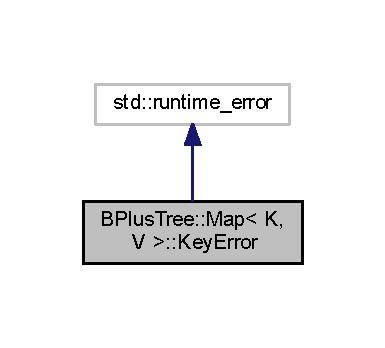
\includegraphics[width=185pt]{class_b_plus_tree_1_1_map_1_1_key_error__inherit__graph}
\end{center}
\end{figure}


Collaboration diagram for B\+Plus\+Tree\+:\+:Map$<$ K, V $>$\+:\+:Key\+Error\+:
\nopagebreak
\begin{figure}[H]
\begin{center}
\leavevmode
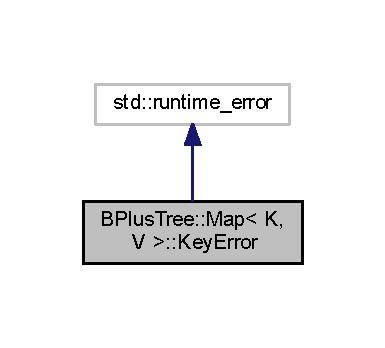
\includegraphics[width=185pt]{class_b_plus_tree_1_1_map_1_1_key_error__coll__graph}
\end{center}
\end{figure}
\subsection*{Public Member Functions}
\begin{DoxyCompactItemize}
\item 
\hyperlink{class_b_plus_tree_1_1_map_1_1_key_error_a9cc95d98613dc60ed60d6da28d912918}{Key\+Error} (std\+::string msg)  throw ()
\item 
\mbox{\Hypertarget{class_b_plus_tree_1_1_map_1_1_key_error_a4200fad129e5831436b936fae48c7b3d}\label{class_b_plus_tree_1_1_map_1_1_key_error_a4200fad129e5831436b936fae48c7b3d}} 
const char $\ast$ {\bfseries what} () const  throw ()
\end{DoxyCompactItemize}


\subsection{Constructor \& Destructor Documentation}
\mbox{\Hypertarget{class_b_plus_tree_1_1_map_1_1_key_error_a9cc95d98613dc60ed60d6da28d912918}\label{class_b_plus_tree_1_1_map_1_1_key_error_a9cc95d98613dc60ed60d6da28d912918}} 
\index{B\+Plus\+Tree\+::\+Map\+::\+Key\+Error@{B\+Plus\+Tree\+::\+Map\+::\+Key\+Error}!Key\+Error@{Key\+Error}}
\index{Key\+Error@{Key\+Error}!B\+Plus\+Tree\+::\+Map\+::\+Key\+Error@{B\+Plus\+Tree\+::\+Map\+::\+Key\+Error}}
\subsubsection{\texorpdfstring{Key\+Error()}{KeyError()}}
{\footnotesize\ttfamily template$<$typename K , typename V $>$ \\
\hyperlink{class_b_plus_tree_1_1_map}{B\+Plus\+Tree\+::\+Map}$<$ K, V $>$\+::Key\+Error\+::\+Key\+Error (\begin{DoxyParamCaption}\item[{std\+::string}]{msg }\end{DoxyParamCaption}) throw  ) \hspace{0.3cm}{\ttfamily [inline]}}

Map\+::\+Key Error


\begin{DoxyExceptions}{Exceptions}
{\em msg} & \\
\hline
\end{DoxyExceptions}

\begin{DoxyParams}{Parameters}
{\em msg} & \\
\hline
\end{DoxyParams}


The documentation for this class was generated from the following file\+:\begin{DoxyCompactItemize}
\item 
include/bptree.\+h\end{DoxyCompactItemize}

\hypertarget{class_b_plus_tree_1_1_map}{}\section{B\+Plus\+Tree\+:\+:Map$<$ K, V $>$ Class Template Reference}
\label{class_b_plus_tree_1_1_map}\index{B\+Plus\+Tree\+::\+Map$<$ K, V $>$@{B\+Plus\+Tree\+::\+Map$<$ K, V $>$}}
\subsection*{Classes}
\begin{DoxyCompactItemize}
\item 
class \hyperlink{class_b_plus_tree_1_1_map_1_1_key_error}{Key\+Error}
\end{DoxyCompactItemize}
\subsection*{Public Member Functions}
\begin{DoxyCompactItemize}
\item 
\mbox{\Hypertarget{class_b_plus_tree_1_1_map_ae4b13c6da4151d439ec19618cfb1bab4}\label{class_b_plus_tree_1_1_map_ae4b13c6da4151d439ec19618cfb1bab4}} 
{\bfseries Map} (int degree)  throw ()
\item 
void \hyperlink{class_b_plus_tree_1_1_map_ab29d127d6b90f8f7c84270d4f1c034f9}{set} (K key, V value)  throw ()
\item 
V \hyperlink{class_b_plus_tree_1_1_map_a28d991d412dd816530c8509274d48a0a}{get} (K key) const
\item 
\mbox{\Hypertarget{class_b_plus_tree_1_1_map_aaefa90cc584499c4ff4ee8f2d332b764}\label{class_b_plus_tree_1_1_map_aaefa90cc584499c4ff4ee8f2d332b764}} 
V {\bfseries get} (K key, V default\+\_\+) const  throw ()
\item 
void \hyperlink{class_b_plus_tree_1_1_map_a99b2e74d5c38e0e27fe8031e1f9990f8}{remove} (K key)  throw ()
\end{DoxyCompactItemize}
\subsection*{Public Attributes}
\begin{DoxyCompactItemize}
\item 
\mbox{\Hypertarget{class_b_plus_tree_1_1_map_a8d26aa7480f3cfbdf35e3cd02cea6bbf}\label{class_b_plus_tree_1_1_map_a8d26aa7480f3cfbdf35e3cd02cea6bbf}} 
const int {\bfseries degree}
\end{DoxyCompactItemize}


\subsection{Member Function Documentation}
\mbox{\Hypertarget{class_b_plus_tree_1_1_map_a28d991d412dd816530c8509274d48a0a}\label{class_b_plus_tree_1_1_map_a28d991d412dd816530c8509274d48a0a}} 
\index{B\+Plus\+Tree\+::\+Map@{B\+Plus\+Tree\+::\+Map}!get@{get}}
\index{get@{get}!B\+Plus\+Tree\+::\+Map@{B\+Plus\+Tree\+::\+Map}}
\subsubsection{\texorpdfstring{get()}{get()}}
{\footnotesize\ttfamily template$<$typename K , typename V $>$ \\
V \hyperlink{class_b_plus_tree_1_1_map}{B\+Plus\+Tree\+::\+Map}$<$ K, V $>$\+::get (\begin{DoxyParamCaption}\item[{K}]{key }\end{DoxyParamCaption}) const}

\hyperlink{class_b_plus_tree_1_1_map_a28d991d412dd816530c8509274d48a0a}{Map\+::get} key


\begin{DoxyParams}{Parameters}
{\em key} & \\
\hline
\end{DoxyParams}
\mbox{\Hypertarget{class_b_plus_tree_1_1_map_a99b2e74d5c38e0e27fe8031e1f9990f8}\label{class_b_plus_tree_1_1_map_a99b2e74d5c38e0e27fe8031e1f9990f8}} 
\index{B\+Plus\+Tree\+::\+Map@{B\+Plus\+Tree\+::\+Map}!remove@{remove}}
\index{remove@{remove}!B\+Plus\+Tree\+::\+Map@{B\+Plus\+Tree\+::\+Map}}
\subsubsection{\texorpdfstring{remove()}{remove()}}
{\footnotesize\ttfamily template$<$typename K , typename V $>$ \\
void \hyperlink{class_b_plus_tree_1_1_map}{B\+Plus\+Tree\+::\+Map}$<$ K, V $>$\+::remove (\begin{DoxyParamCaption}\item[{K}]{key }\end{DoxyParamCaption}) throw  ) }

Map\+::\+Remove key


\begin{DoxyParams}{Parameters}
{\em key} & \\
\hline
\end{DoxyParams}

\begin{DoxyExceptions}{Exceptions}
{\em } & \\
\hline
\end{DoxyExceptions}
\mbox{\Hypertarget{class_b_plus_tree_1_1_map_ab29d127d6b90f8f7c84270d4f1c034f9}\label{class_b_plus_tree_1_1_map_ab29d127d6b90f8f7c84270d4f1c034f9}} 
\index{B\+Plus\+Tree\+::\+Map@{B\+Plus\+Tree\+::\+Map}!set@{set}}
\index{set@{set}!B\+Plus\+Tree\+::\+Map@{B\+Plus\+Tree\+::\+Map}}
\subsubsection{\texorpdfstring{set()}{set()}}
{\footnotesize\ttfamily template$<$typename K , typename V $>$ \\
void \hyperlink{class_b_plus_tree_1_1_map}{B\+Plus\+Tree\+::\+Map}$<$ K, V $>$\+::set (\begin{DoxyParamCaption}\item[{K}]{key,  }\item[{V}]{value }\end{DoxyParamCaption}) throw  ) }

\hyperlink{class_b_plus_tree_1_1_map_ab29d127d6b90f8f7c84270d4f1c034f9}{Map\+::set}


\begin{DoxyParams}{Parameters}
{\em key} & \\
\hline
{\em value} & \\
\hline
\end{DoxyParams}

\begin{DoxyExceptions}{Exceptions}
{\em } & \\
\hline
\end{DoxyExceptions}


The documentation for this class was generated from the following file\+:\begin{DoxyCompactItemize}
\item 
include/bptree.\+h\end{DoxyCompactItemize}

\hypertarget{struct_b_plus_tree_1_1_node}{}\section{B\+Plus\+Tree\+:\+:Node$<$ K, V $>$ Struct Template Reference}
\label{struct_b_plus_tree_1_1_node}\index{B\+Plus\+Tree\+::\+Node$<$ K, V $>$@{B\+Plus\+Tree\+::\+Node$<$ K, V $>$}}
\subsection*{Public Attributes}
\begin{DoxyCompactItemize}
\item 
\mbox{\Hypertarget{struct_b_plus_tree_1_1_node_a86fcd3fb476654ff940932e5a0727497}\label{struct_b_plus_tree_1_1_node_a86fcd3fb476654ff940932e5a0727497}} 
std\+::vector$<$ K $>$ {\bfseries keys}
\item 
\mbox{\Hypertarget{struct_b_plus_tree_1_1_node_a837f51e703d489dfc8f326a262c8d3ba}\label{struct_b_plus_tree_1_1_node_a837f51e703d489dfc8f326a262c8d3ba}} 
std\+::vector$<$ \hyperlink{struct_b_plus_tree_1_1_node}{Node}$<$ K, V $>$ $>$ {\bfseries edges}
\item 
\mbox{\Hypertarget{struct_b_plus_tree_1_1_node_a09ff79beef41471d1e273c46f55c2fc9}\label{struct_b_plus_tree_1_1_node_a09ff79beef41471d1e273c46f55c2fc9}} 
std\+::vector$<$ V $>$ {\bfseries values}
\end{DoxyCompactItemize}


The documentation for this struct was generated from the following file\+:\begin{DoxyCompactItemize}
\item 
include/bptree.\+h\end{DoxyCompactItemize}

\hypertarget{class_database_1_1_query}{}\section{Database\+:\+:Query Class Reference}
\label{class_database_1_1_query}\index{Database\+::\+Query@{Database\+::\+Query}}
\subsection*{Public Member Functions}
\begin{DoxyCompactItemize}
\item 
\mbox{\Hypertarget{class_database_1_1_query_ad5836c20a5d0611b8d6cdacdc228057f}\label{class_database_1_1_query_ad5836c20a5d0611b8d6cdacdc228057f}} 
{\bfseries Query} (const \hyperlink{class_database}{Database} \&db)
\item 
const \hyperlink{class_database_1_1_query}{Query} \& \hyperlink{class_database_1_1_query_a020ff17d626e968eb94c7f6932d375a4}{select} (std\+::string key)
\item 
const \hyperlink{class_database_1_1_query}{Query} \& \hyperlink{class_database_1_1_query_a331879c9d479b94cf19c79b9b3a2eddc}{set\+\_\+option} (Query\+Option\+Type opt, \hyperlink{union_query_option_data}{Query\+Option\+Data} value)
\item 
const \hyperlink{class_database_1_1_query}{Query} \& \hyperlink{class_database_1_1_query_a920f38ec4ae0d11a1792e4c412506cb2}{order\+\_\+by} (std\+::string key)
\item 
\mbox{\Hypertarget{class_database_1_1_query_a556b41f8b42a631adec49f70da8ef9b9}\label{class_database_1_1_query_a556b41f8b42a631adec49f70da8ef9b9}} 
\hyperlink{class_database}{Database} {\bfseries all} ()
\end{DoxyCompactItemize}


\subsection{Member Function Documentation}
\mbox{\Hypertarget{class_database_1_1_query_a920f38ec4ae0d11a1792e4c412506cb2}\label{class_database_1_1_query_a920f38ec4ae0d11a1792e4c412506cb2}} 
\index{Database\+::\+Query@{Database\+::\+Query}!order\+\_\+by@{order\+\_\+by}}
\index{order\+\_\+by@{order\+\_\+by}!Database\+::\+Query@{Database\+::\+Query}}
\subsubsection{\texorpdfstring{order\+\_\+by()}{order\_by()}}
{\footnotesize\ttfamily const \hyperlink{class_database_1_1_query}{Query}\& Database\+::\+Query\+::order\+\_\+by (\begin{DoxyParamCaption}\item[{std\+::string}]{key }\end{DoxyParamCaption})}

\hyperlink{class_database_1_1_query_a920f38ec4ae0d11a1792e4c412506cb2}{Query\+::order\+\_\+by}


\begin{DoxyParams}{Parameters}
{\em key} & Order by given key \\
\hline
\end{DoxyParams}
\mbox{\Hypertarget{class_database_1_1_query_a020ff17d626e968eb94c7f6932d375a4}\label{class_database_1_1_query_a020ff17d626e968eb94c7f6932d375a4}} 
\index{Database\+::\+Query@{Database\+::\+Query}!select@{select}}
\index{select@{select}!Database\+::\+Query@{Database\+::\+Query}}
\subsubsection{\texorpdfstring{select()}{select()}}
{\footnotesize\ttfamily const \hyperlink{class_database_1_1_query}{Query}\& Database\+::\+Query\+::select (\begin{DoxyParamCaption}\item[{std\+::string}]{key }\end{DoxyParamCaption})}

\hyperlink{class_database_1_1_query_a020ff17d626e968eb94c7f6932d375a4}{Query\+::select}


\begin{DoxyParams}{Parameters}
{\em key} & A string \\
\hline
\end{DoxyParams}
\mbox{\Hypertarget{class_database_1_1_query_a331879c9d479b94cf19c79b9b3a2eddc}\label{class_database_1_1_query_a331879c9d479b94cf19c79b9b3a2eddc}} 
\index{Database\+::\+Query@{Database\+::\+Query}!set\+\_\+option@{set\+\_\+option}}
\index{set\+\_\+option@{set\+\_\+option}!Database\+::\+Query@{Database\+::\+Query}}
\subsubsection{\texorpdfstring{set\+\_\+option()}{set\_option()}}
{\footnotesize\ttfamily const \hyperlink{class_database_1_1_query}{Query}\& Database\+::\+Query\+::set\+\_\+option (\begin{DoxyParamCaption}\item[{Query\+Option\+Type}]{opt,  }\item[{\hyperlink{union_query_option_data}{Query\+Option\+Data}}]{value }\end{DoxyParamCaption})}

\hyperlink{class_database_1_1_query_a331879c9d479b94cf19c79b9b3a2eddc}{Query\+::set\+\_\+option} \hyperlink{struct_field}{Field}


\begin{DoxyParams}{Parameters}
{\em opt} & \hyperlink{class_database_1_1_query}{Query} option type \\
\hline
{\em value} & \hyperlink{class_database_1_1_query}{Query} option data value \\
\hline
\end{DoxyParams}


The documentation for this class was generated from the following file\+:\begin{DoxyCompactItemize}
\item 
include/database.\+h\end{DoxyCompactItemize}

\hypertarget{union_query_option_data}{}\section{Query\+Option\+Data Union Reference}
\label{union_query_option_data}\index{Query\+Option\+Data@{Query\+Option\+Data}}
\subsection*{Public Attributes}
\begin{DoxyCompactItemize}
\item 
\mbox{\Hypertarget{union_query_option_data_aff4c9bdf206c01994c797a119c922fa9}\label{union_query_option_data_aff4c9bdf206c01994c797a119c922fa9}} 
int {\bfseries capacity}
\end{DoxyCompactItemize}


The documentation for this union was generated from the following file\+:\begin{DoxyCompactItemize}
\item 
include/database.\+h\end{DoxyCompactItemize}

\hypertarget{class_database_1_1_record}{}\section{Database\+:\+:Record Class Reference}
\label{class_database_1_1_record}\index{Database\+::\+Record@{Database\+::\+Record}}
\subsection*{Public Member Functions}
\begin{DoxyCompactItemize}
\item 
\hyperlink{class_database_1_1_record_a913e37db1858bc8832c4c647c85268ac}{Record} (const \hyperlink{class_database}{Database} \&db, int row)
\end{DoxyCompactItemize}


\subsection{Constructor \& Destructor Documentation}
\mbox{\Hypertarget{class_database_1_1_record_a913e37db1858bc8832c4c647c85268ac}\label{class_database_1_1_record_a913e37db1858bc8832c4c647c85268ac}} 
\index{Database\+::\+Record@{Database\+::\+Record}!Record@{Record}}
\index{Record@{Record}!Database\+::\+Record@{Database\+::\+Record}}
\subsubsection{\texorpdfstring{Record()}{Record()}}
{\footnotesize\ttfamily Database\+::\+Record\+::\+Record (\begin{DoxyParamCaption}\item[{const \hyperlink{class_database}{Database} \&}]{db,  }\item[{int}]{row }\end{DoxyParamCaption})}

\hyperlink{class_database_1_1_record_a913e37db1858bc8832c4c647c85268ac}{Database\+::\+Record\+::\+Record}


\begin{DoxyParams}{Parameters}
{\em db} & \hyperlink{class_database}{Database} \\
\hline
{\em row} & Row number \\
\hline
\end{DoxyParams}


The documentation for this class was generated from the following file\+:\begin{DoxyCompactItemize}
\item 
include/database.\+h\end{DoxyCompactItemize}

\hypertarget{class_collection_1_1_record}{}\section{Collection\+:\+:Record Class Reference}
\label{class_collection_1_1_record}\index{Collection\+::\+Record@{Collection\+::\+Record}}
\subsection*{Public Member Functions}
\begin{DoxyCompactItemize}
\item 
\hyperlink{struct_field}{Field} \hyperlink{class_collection_1_1_record_ac045539ed42788b33b56c0c60b4bede4}{get} (std\+::string key\+\_\+name)
\item 
\hyperlink{struct_field}{Field} \hyperlink{class_collection_1_1_record_a7e977898edd578a4dd198798e77c96c7}{get} (\hyperlink{struct_key}{Key} key)
\item 
\mbox{\Hypertarget{class_collection_1_1_record_a74ccccdc99f2a9bd9ee79d7b24b12637}\label{class_collection_1_1_record_a74ccccdc99f2a9bd9ee79d7b24b12637}} 
\hyperlink{struct_field}{Field} {\bfseries operator\mbox{[}$\,$\mbox{]}} (std\+::string key\+\_\+name)
\item 
\mbox{\Hypertarget{class_collection_1_1_record_a1d1f629974dd996feddf5ddb9d15c689}\label{class_collection_1_1_record_a1d1f629974dd996feddf5ddb9d15c689}} 
\hyperlink{struct_field}{Field} {\bfseries operator\mbox{[}$\,$\mbox{]}} (\hyperlink{struct_key}{Key} key)
\item 
\mbox{\Hypertarget{class_collection_1_1_record_ae5891a93674f570c9b30e2d6eee381a8}\label{class_collection_1_1_record_ae5891a93674f570c9b30e2d6eee381a8}} 
bool {\bfseries lt} (\hyperlink{class_collection_1_1_record}{Record} \&other, std\+::vector$<$ \hyperlink{struct_key}{Key} $>$ \hyperlink{class_collection_aebff0d78673dac8453ebf51ba32d10eb}{keys})
\item 
\mbox{\Hypertarget{class_collection_1_1_record_a5f1321a0fd4f5ef2570917d2c3407a90}\label{class_collection_1_1_record_a5f1321a0fd4f5ef2570917d2c3407a90}} 
bool {\bfseries lte} (\hyperlink{class_collection_1_1_record}{Record} \&other, std\+::vector$<$ \hyperlink{struct_key}{Key} $>$ \hyperlink{class_collection_aebff0d78673dac8453ebf51ba32d10eb}{keys})
\item 
\mbox{\Hypertarget{class_collection_1_1_record_ad9f0b6f2e1bb15e922d54280eaad85bf}\label{class_collection_1_1_record_ad9f0b6f2e1bb15e922d54280eaad85bf}} 
bool {\bfseries gt} (\hyperlink{class_collection_1_1_record}{Record} \&other, std\+::vector$<$ \hyperlink{struct_key}{Key} $>$ \hyperlink{class_collection_aebff0d78673dac8453ebf51ba32d10eb}{keys})
\item 
\mbox{\Hypertarget{class_collection_1_1_record_a27aca1d2127efc59562ffd47e381249e}\label{class_collection_1_1_record_a27aca1d2127efc59562ffd47e381249e}} 
bool {\bfseries gte} (\hyperlink{class_collection_1_1_record}{Record} \&other, std\+::vector$<$ \hyperlink{struct_key}{Key} $>$ \hyperlink{class_collection_aebff0d78673dac8453ebf51ba32d10eb}{keys})
\item 
\mbox{\Hypertarget{class_collection_1_1_record_affc0e1f2bc3d8d5e92338f186fc2d1f7}\label{class_collection_1_1_record_affc0e1f2bc3d8d5e92338f186fc2d1f7}} 
std\+::string {\bfseries str} ()
\end{DoxyCompactItemize}
\subsection*{Public Attributes}
\begin{DoxyCompactItemize}
\item 
const size\+\_\+t \hyperlink{class_collection_1_1_record_aabb05802a9c94e791df47bd7d8bda096}{offset}
\end{DoxyCompactItemize}
\subsection*{Friends}
\begin{DoxyCompactItemize}
\item 
\mbox{\Hypertarget{class_collection_1_1_record_a6e332922765a19fc2a9593a20f26fc95}\label{class_collection_1_1_record_a6e332922765a19fc2a9593a20f26fc95}} 
class {\bfseries Collection}
\end{DoxyCompactItemize}


\subsection{Member Function Documentation}
\mbox{\Hypertarget{class_collection_1_1_record_ac045539ed42788b33b56c0c60b4bede4}\label{class_collection_1_1_record_ac045539ed42788b33b56c0c60b4bede4}} 
\index{Collection\+::\+Record@{Collection\+::\+Record}!get@{get}}
\index{get@{get}!Collection\+::\+Record@{Collection\+::\+Record}}
\subsubsection{\texorpdfstring{get()}{get()}\hspace{0.1cm}{\footnotesize\ttfamily [1/2]}}
{\footnotesize\ttfamily \hyperlink{struct_field}{Field} Collection\+::\+Record\+::get (\begin{DoxyParamCaption}\item[{std\+::string}]{key\+\_\+name }\end{DoxyParamCaption})}

Finds key name and gets key


\begin{DoxyParams}{Parameters}
{\em key\+\_\+name} & \\
\hline
\end{DoxyParams}
\begin{DoxyReturn}{Returns}
Collection\+::\+Record\+::get(key) 
\end{DoxyReturn}
\mbox{\Hypertarget{class_collection_1_1_record_a7e977898edd578a4dd198798e77c96c7}\label{class_collection_1_1_record_a7e977898edd578a4dd198798e77c96c7}} 
\index{Collection\+::\+Record@{Collection\+::\+Record}!get@{get}}
\index{get@{get}!Collection\+::\+Record@{Collection\+::\+Record}}
\subsubsection{\texorpdfstring{get()}{get()}\hspace{0.1cm}{\footnotesize\ttfamily [2/2]}}
{\footnotesize\ttfamily \hyperlink{struct_field}{Field} Collection\+::\+Record\+::get (\begin{DoxyParamCaption}\item[{\hyperlink{struct_key}{Key}}]{key }\end{DoxyParamCaption})}

Gets key from field in record


\begin{DoxyParams}{Parameters}
{\em key} & \\
\hline
\end{DoxyParams}


\subsection{Member Data Documentation}
\mbox{\Hypertarget{class_collection_1_1_record_aabb05802a9c94e791df47bd7d8bda096}\label{class_collection_1_1_record_aabb05802a9c94e791df47bd7d8bda096}} 
\index{Collection\+::\+Record@{Collection\+::\+Record}!offset@{offset}}
\index{offset@{offset}!Collection\+::\+Record@{Collection\+::\+Record}}
\subsubsection{\texorpdfstring{offset}{offset}}
{\footnotesize\ttfamily const size\+\_\+t Collection\+::\+Record\+::offset}

\hyperlink{class_collection_1_1_record_aabb05802a9c94e791df47bd7d8bda096}{Collection\+::\+Record\+::offset} is the offset of the record. 

The documentation for this class was generated from the following file\+:\begin{DoxyCompactItemize}
\item 
include/collection.\+h\end{DoxyCompactItemize}

%--- End generated contents ---

% Index
\backmatter
\newpage
\phantomsection
\clearemptydoublepage
\addcontentsline{toc}{chapter}{Index}
\printindex

\end{document}
